\documentclass[twoside]{book}

% Packages required by doxygen
\usepackage{fixltx2e}
\usepackage{calc}
\usepackage{doxygen}
\usepackage[export]{adjustbox} % also loads graphicx
\usepackage{graphicx}
\usepackage[utf8]{inputenc}
\usepackage{makeidx}
\usepackage{multicol}
\usepackage{multirow}
\PassOptionsToPackage{warn}{textcomp}
\usepackage{textcomp}
\usepackage[nointegrals]{wasysym}
\usepackage[table]{xcolor}

% Font selection
\usepackage[T1]{fontenc}
\usepackage[scaled=.90]{helvet}
\usepackage{courier}
\usepackage{amssymb}
\usepackage{sectsty}
\renewcommand{\familydefault}{\sfdefault}
\allsectionsfont{%
  \fontseries{bc}\selectfont%
  \color{darkgray}%
}
\renewcommand{\DoxyLabelFont}{%
  \fontseries{bc}\selectfont%
  \color{darkgray}%
}
\newcommand{\+}{\discretionary{\mbox{\scriptsize$\hookleftarrow$}}{}{}}

% Page & text layout
\usepackage{geometry}
\geometry{%
  a4paper,%
  top=2.5cm,%
  bottom=2.5cm,%
  left=2.5cm,%
  right=2.5cm%
}
\tolerance=750
\hfuzz=15pt
\hbadness=750
\setlength{\emergencystretch}{15pt}
\setlength{\parindent}{0cm}
\setlength{\parskip}{3ex plus 2ex minus 2ex}
\makeatletter
\renewcommand{\paragraph}{%
  \@startsection{paragraph}{4}{0ex}{-1.0ex}{1.0ex}{%
    \normalfont\normalsize\bfseries\SS@parafont%
  }%
}
\renewcommand{\subparagraph}{%
  \@startsection{subparagraph}{5}{0ex}{-1.0ex}{1.0ex}{%
    \normalfont\normalsize\bfseries\SS@subparafont%
  }%
}
\makeatother

% Headers & footers
\usepackage{fancyhdr}
\pagestyle{fancyplain}
\fancyhead[LE]{\fancyplain{}{\bfseries\thepage}}
\fancyhead[CE]{\fancyplain{}{}}
\fancyhead[RE]{\fancyplain{}{\bfseries\leftmark}}
\fancyhead[LO]{\fancyplain{}{\bfseries\rightmark}}
\fancyhead[CO]{\fancyplain{}{}}
\fancyhead[RO]{\fancyplain{}{\bfseries\thepage}}
\fancyfoot[LE]{\fancyplain{}{}}
\fancyfoot[CE]{\fancyplain{}{}}
\fancyfoot[RE]{\fancyplain{}{\bfseries\scriptsize Generated by Doxygen }}
\fancyfoot[LO]{\fancyplain{}{\bfseries\scriptsize Generated by Doxygen }}
\fancyfoot[CO]{\fancyplain{}{}}
\fancyfoot[RO]{\fancyplain{}{}}
\renewcommand{\footrulewidth}{0.4pt}
\renewcommand{\chaptermark}[1]{%
  \markboth{#1}{}%
}
\renewcommand{\sectionmark}[1]{%
  \markright{\thesection\ #1}%
}

% Indices & bibliography
\usepackage{natbib}
\usepackage[titles]{tocloft}
\setcounter{tocdepth}{3}
\setcounter{secnumdepth}{5}
\makeindex

% Hyperlinks (required, but should be loaded last)
\usepackage{ifpdf}
\ifpdf
  \usepackage[pdftex,pagebackref=true]{hyperref}
\else
  \usepackage[ps2pdf,pagebackref=true]{hyperref}
\fi
\hypersetup{%
  colorlinks=true,%
  linkcolor=blue,%
  citecolor=blue,%
  unicode%
}

% Custom commands
\newcommand{\clearemptydoublepage}{%
  \newpage{\pagestyle{empty}\cleardoublepage}%
}

\usepackage{caption}
\captionsetup{labelsep=space,justification=centering,font={bf},singlelinecheck=off,skip=4pt,position=top}

%===== C O N T E N T S =====

\begin{document}

% Titlepage & ToC
\hypersetup{pageanchor=false,
             bookmarksnumbered=true,
             pdfencoding=unicode
            }
\pagenumbering{alph}
\begin{titlepage}
\vspace*{7cm}
\begin{center}%
{\Large My Project }\\
\vspace*{1cm}
{\large Generated by Doxygen 1.8.15}\\
\end{center}
\end{titlepage}
\clearemptydoublepage
\pagenumbering{roman}
\tableofcontents
\clearemptydoublepage
\pagenumbering{arabic}
\hypersetup{pageanchor=true}

%--- Begin generated contents ---
\chapter{Hierarchical Index}
\section{Class Hierarchy}
This inheritance list is sorted roughly, but not completely, alphabetically\+:\begin{DoxyCompactList}
\item \contentsline{section}{Customer\+Item}{\pageref{classCustomerItem}}{}
\item \contentsline{section}{Customer\+Order}{\pageref{classCustomerOrder}}{}
\item \contentsline{section}{Item}{\pageref{classItem}}{}
\item \contentsline{section}{Task}{\pageref{classTask}}{}
\item \contentsline{section}{Utilities}{\pageref{classUtilities}}{}
\item vector\begin{DoxyCompactList}
\item \contentsline{section}{Item\+Manager}{\pageref{classItemManager}}{}
\item \contentsline{section}{Order\+Manager}{\pageref{classOrderManager}}{}
\item \contentsline{section}{Task\+Manager}{\pageref{classTaskManager}}{}
\end{DoxyCompactList}
\end{DoxyCompactList}

\chapter{Class Index}
\section{Class List}
Here are the classes, structs, unions and interfaces with brief descriptions\+:\begin{DoxyCompactList}
\item\contentsline{section}{\mbox{\hyperlink{classw8_1_1DataTable}{w8\+::\+Data\+Table$<$ T $>$}} }{\pageref{classw8_1_1DataTable}}{}
\end{DoxyCompactList}

\chapter{Class Documentation}
\hypertarget{classCustomerItem}{}\section{Customer\+Item Class Reference}
\label{classCustomerItem}\index{Customer\+Item@{Customer\+Item}}
\subsection*{Public Member Functions}
\begin{DoxyCompactItemize}
\item 
\mbox{\hyperlink{classCustomerItem_a7868c9be14aced9e5e6f657a0e5671fc}{Customer\+Item}} (const std\+::string \&=std\+::string())
\item 
bool \mbox{\hyperlink{classCustomerItem_a6275dac4b75e3cd8e56f504140cd135d}{asks\+For}} (const \mbox{\hyperlink{classItem}{Item}} \&) const
\item 
bool \mbox{\hyperlink{classCustomerItem_a39f6b78f595b7d4a20f1e7f945834335}{is\+Filled}} () const
\item 
void \mbox{\hyperlink{classCustomerItem_a31c01c091f1ebc623a66d80235bc5e8c}{fill}} (const unsigned int)
\item 
void \mbox{\hyperlink{classCustomerItem_af6a25490940dcac3842f877ea0da4580}{clear}} ()
\item 
const std\+::string \& \mbox{\hyperlink{classCustomerItem_a7922e8405fdcfff7ca45decd2a54efdc}{get\+Name}} () const
\item 
void \mbox{\hyperlink{classCustomerItem_a2aaa8551a3662bb4b2953704580fc408}{display}} (std\+::ostream \&) const
\end{DoxyCompactItemize}


\subsection{Constructor \& Destructor Documentation}
\mbox{\Hypertarget{classCustomerItem_a7868c9be14aced9e5e6f657a0e5671fc}\label{classCustomerItem_a7868c9be14aced9e5e6f657a0e5671fc}} 
\index{Customer\+Item@{Customer\+Item}!Customer\+Item@{Customer\+Item}}
\index{Customer\+Item@{Customer\+Item}!Customer\+Item@{Customer\+Item}}
\subsubsection{\texorpdfstring{Customer\+Item()}{CustomerItem()}}
{\footnotesize\ttfamily Customer\+Item\+::\+Customer\+Item (\begin{DoxyParamCaption}\item[{const std\+::string \&}]{str = {\ttfamily std\+:\+:string()} }\end{DoxyParamCaption})}

Constructor that builds a \mbox{\hyperlink{classCustomerItem}{Customer\+Item}} object using a string object parameter 

\subsection{Member Function Documentation}
\mbox{\Hypertarget{classCustomerItem_a6275dac4b75e3cd8e56f504140cd135d}\label{classCustomerItem_a6275dac4b75e3cd8e56f504140cd135d}} 
\index{Customer\+Item@{Customer\+Item}!asks\+For@{asks\+For}}
\index{asks\+For@{asks\+For}!Customer\+Item@{Customer\+Item}}
\subsubsection{\texorpdfstring{asks\+For()}{asksFor()}}
{\footnotesize\ttfamily bool Customer\+Item\+::asks\+For (\begin{DoxyParamCaption}\item[{const \mbox{\hyperlink{classItem}{Item}} \&}]{x }\end{DoxyParamCaption}) const}

Query member function that returns true if the current object\textquotesingle{}s name is equal to the \mbox{\hyperlink{classItem}{Item}} object reference parameter \mbox{\Hypertarget{classCustomerItem_af6a25490940dcac3842f877ea0da4580}\label{classCustomerItem_af6a25490940dcac3842f877ea0da4580}} 
\index{Customer\+Item@{Customer\+Item}!clear@{clear}}
\index{clear@{clear}!Customer\+Item@{Customer\+Item}}
\subsubsection{\texorpdfstring{clear()}{clear()}}
{\footnotesize\ttfamily void Customer\+Item\+::clear (\begin{DoxyParamCaption}{ }\end{DoxyParamCaption})}

Member function that sets the object in an empty state \mbox{\Hypertarget{classCustomerItem_a2aaa8551a3662bb4b2953704580fc408}\label{classCustomerItem_a2aaa8551a3662bb4b2953704580fc408}} 
\index{Customer\+Item@{Customer\+Item}!display@{display}}
\index{display@{display}!Customer\+Item@{Customer\+Item}}
\subsubsection{\texorpdfstring{display()}{display()}}
{\footnotesize\ttfamily void Customer\+Item\+::display (\begin{DoxyParamCaption}\item[{std\+::ostream \&}]{os }\end{DoxyParamCaption}) const}

Query member function that displays the object\textquotesingle{}s details to the referenced ostream object parameter \mbox{\Hypertarget{classCustomerItem_a31c01c091f1ebc623a66d80235bc5e8c}\label{classCustomerItem_a31c01c091f1ebc623a66d80235bc5e8c}} 
\index{Customer\+Item@{Customer\+Item}!fill@{fill}}
\index{fill@{fill}!Customer\+Item@{Customer\+Item}}
\subsubsection{\texorpdfstring{fill()}{fill()}}
{\footnotesize\ttfamily void Customer\+Item\+::fill (\begin{DoxyParamCaption}\item[{const unsigned int}]{item\+Code }\end{DoxyParamCaption})}

Member function that sets filled to true and sets the item code to the parametered unsigned integer \mbox{\Hypertarget{classCustomerItem_a7922e8405fdcfff7ca45decd2a54efdc}\label{classCustomerItem_a7922e8405fdcfff7ca45decd2a54efdc}} 
\index{Customer\+Item@{Customer\+Item}!get\+Name@{get\+Name}}
\index{get\+Name@{get\+Name}!Customer\+Item@{Customer\+Item}}
\subsubsection{\texorpdfstring{get\+Name()}{getName()}}
{\footnotesize\ttfamily const std\+::string \& Customer\+Item\+::get\+Name (\begin{DoxyParamCaption}{ }\end{DoxyParamCaption}) const}

Query member function that returns the string object referencing this object\textquotesingle{}s name \mbox{\Hypertarget{classCustomerItem_a39f6b78f595b7d4a20f1e7f945834335}\label{classCustomerItem_a39f6b78f595b7d4a20f1e7f945834335}} 
\index{Customer\+Item@{Customer\+Item}!is\+Filled@{is\+Filled}}
\index{is\+Filled@{is\+Filled}!Customer\+Item@{Customer\+Item}}
\subsubsection{\texorpdfstring{is\+Filled()}{isFilled()}}
{\footnotesize\ttfamily bool Customer\+Item\+::is\+Filled (\begin{DoxyParamCaption}{ }\end{DoxyParamCaption}) const}

Query member function that returns the status of the object\textquotesingle{}s request 

The documentation for this class was generated from the following files\+:\begin{DoxyCompactItemize}
\item 
Customer\+Item.\+h\item 
Customer\+Item.\+cpp\end{DoxyCompactItemize}

\hypertarget{classCustomerOrder}{}\section{Customer\+Order Class Reference}
\label{classCustomerOrder}\index{Customer\+Order@{Customer\+Order}}
\subsection*{Public Member Functions}
\begin{DoxyCompactItemize}
\item 
\mbox{\hyperlink{classCustomerOrder_a0b43beee099ac2772cadd8f3df890701}{Customer\+Order}} (const std\+::string \&)
\item 
\mbox{\hyperlink{classCustomerOrder_ad5d7da49c28e5006f326e1709b072516}{Customer\+Order}} (const \mbox{\hyperlink{classCustomerOrder}{Customer\+Order}} \&)
\item 
\mbox{\hyperlink{classCustomerOrder}{Customer\+Order}} \& \mbox{\hyperlink{classCustomerOrder_ae43fcf650924cf82800c6dfe9a20afca}{operator=}} (const \mbox{\hyperlink{classCustomerOrder}{Customer\+Order}} \&)=delete
\item 
\mbox{\hyperlink{classCustomerOrder_addc080f9b7685c1c2d788b418bca40a8}{Customer\+Order}} (\mbox{\hyperlink{classCustomerOrder}{Customer\+Order}} \&\&) N\+O\+E\+X\+C\+E\+PT
\item 
\mbox{\hyperlink{classCustomerOrder}{Customer\+Order}} \&\& \mbox{\hyperlink{classCustomerOrder_aa500234981e09ab8924631d8a74c9fca}{operator=}} (\mbox{\hyperlink{classCustomerOrder}{Customer\+Order}} \&\&) N\+O\+E\+X\+C\+E\+PT
\item 
\mbox{\hyperlink{classCustomerOrder_ae36af98287386c97b66537ac463b09c6}{$\sim$\+Customer\+Order}} ()
\item 
unsigned int \mbox{\hyperlink{classCustomerOrder_a371158bfa7784275a71ebfd9feb8514b}{no\+Orders}} () const
\item 
const std\+::string \& \mbox{\hyperlink{classCustomerOrder_a8ff1239910926e660ce7692807a7847d}{operator\mbox{[}$\,$\mbox{]}}} (unsigned int) const
\item 
void \mbox{\hyperlink{classCustomerOrder_a317213ffac6bc2765e573893bd3f8507}{fill}} (\mbox{\hyperlink{classItem}{Item}} \&)
\item 
void \mbox{\hyperlink{classCustomerOrder_a8059d5a73bfa388f86671d45835468d6}{remove}} (\mbox{\hyperlink{classItem}{Item}} \&)
\item 
bool \mbox{\hyperlink{classCustomerOrder_a8cfde59bf7a044e21508f5b595e3873c}{empty}} () const
\item 
void \mbox{\hyperlink{classCustomerOrder_a44b8223600dd858b4d4edcbe3704a5a0}{display}} (std\+::ostream \&) const
\end{DoxyCompactItemize}


\subsection{Constructor \& Destructor Documentation}
\mbox{\Hypertarget{classCustomerOrder_a0b43beee099ac2772cadd8f3df890701}\label{classCustomerOrder_a0b43beee099ac2772cadd8f3df890701}} 
\index{Customer\+Order@{Customer\+Order}!Customer\+Order@{Customer\+Order}}
\index{Customer\+Order@{Customer\+Order}!Customer\+Order@{Customer\+Order}}
\subsubsection{\texorpdfstring{Customer\+Order()}{CustomerOrder()}\hspace{0.1cm}{\footnotesize\ttfamily [1/3]}}
{\footnotesize\ttfamily Customer\+Order\+::\+Customer\+Order (\begin{DoxyParamCaption}\item[{const std\+::string \&}]{str }\end{DoxyParamCaption})}

Constructor that initializes the object using a string ready to be parsed \mbox{\Hypertarget{classCustomerOrder_ad5d7da49c28e5006f326e1709b072516}\label{classCustomerOrder_ad5d7da49c28e5006f326e1709b072516}} 
\index{Customer\+Order@{Customer\+Order}!Customer\+Order@{Customer\+Order}}
\index{Customer\+Order@{Customer\+Order}!Customer\+Order@{Customer\+Order}}
\subsubsection{\texorpdfstring{Customer\+Order()}{CustomerOrder()}\hspace{0.1cm}{\footnotesize\ttfamily [2/3]}}
{\footnotesize\ttfamily Customer\+Order\+::\+Customer\+Order (\begin{DoxyParamCaption}\item[{const \mbox{\hyperlink{classCustomerOrder}{Customer\+Order}} \&}]{ }\end{DoxyParamCaption})}

Constructor that throws an exception when called as to not create duplications of the same object \mbox{\Hypertarget{classCustomerOrder_addc080f9b7685c1c2d788b418bca40a8}\label{classCustomerOrder_addc080f9b7685c1c2d788b418bca40a8}} 
\index{Customer\+Order@{Customer\+Order}!Customer\+Order@{Customer\+Order}}
\index{Customer\+Order@{Customer\+Order}!Customer\+Order@{Customer\+Order}}
\subsubsection{\texorpdfstring{Customer\+Order()}{CustomerOrder()}\hspace{0.1cm}{\footnotesize\ttfamily [3/3]}}
{\footnotesize\ttfamily Customer\+Order\+::\+Customer\+Order (\begin{DoxyParamCaption}\item[{\mbox{\hyperlink{classCustomerOrder}{Customer\+Order}} \&\&}]{object }\end{DoxyParamCaption})}

Move constructor that uses an R value \mbox{\hyperlink{classCustomerOrder}{Customer\+Order}} object reference to build a \mbox{\hyperlink{classCustomerOrder}{Customer\+Order}} object. \mbox{\Hypertarget{classCustomerOrder_ae36af98287386c97b66537ac463b09c6}\label{classCustomerOrder_ae36af98287386c97b66537ac463b09c6}} 
\index{Customer\+Order@{Customer\+Order}!````~Customer\+Order@{$\sim$\+Customer\+Order}}
\index{````~Customer\+Order@{$\sim$\+Customer\+Order}!Customer\+Order@{Customer\+Order}}
\subsubsection{\texorpdfstring{$\sim$\+Customer\+Order()}{~CustomerOrder()}}
{\footnotesize\ttfamily Customer\+Order\+::$\sim$\+Customer\+Order (\begin{DoxyParamCaption}{ }\end{DoxyParamCaption})}

Destructor that handles the removal of dynamic datatypes 

\subsection{Member Function Documentation}
\mbox{\Hypertarget{classCustomerOrder_a44b8223600dd858b4d4edcbe3704a5a0}\label{classCustomerOrder_a44b8223600dd858b4d4edcbe3704a5a0}} 
\index{Customer\+Order@{Customer\+Order}!display@{display}}
\index{display@{display}!Customer\+Order@{Customer\+Order}}
\subsubsection{\texorpdfstring{display()}{display()}}
{\footnotesize\ttfamily void Customer\+Order\+::display (\begin{DoxyParamCaption}\item[{std\+::ostream \&}]{os }\end{DoxyParamCaption}) const}

Query member function that displays the object\textquotesingle{}s details to the ostream object reference parameter \mbox{\Hypertarget{classCustomerOrder_a8cfde59bf7a044e21508f5b595e3873c}\label{classCustomerOrder_a8cfde59bf7a044e21508f5b595e3873c}} 
\index{Customer\+Order@{Customer\+Order}!empty@{empty}}
\index{empty@{empty}!Customer\+Order@{Customer\+Order}}
\subsubsection{\texorpdfstring{empty()}{empty()}}
{\footnotesize\ttfamily bool Customer\+Order\+::empty (\begin{DoxyParamCaption}{ }\end{DoxyParamCaption}) const}

Query member function that returns true if the current object is empty \mbox{\Hypertarget{classCustomerOrder_a317213ffac6bc2765e573893bd3f8507}\label{classCustomerOrder_a317213ffac6bc2765e573893bd3f8507}} 
\index{Customer\+Order@{Customer\+Order}!fill@{fill}}
\index{fill@{fill}!Customer\+Order@{Customer\+Order}}
\subsubsection{\texorpdfstring{fill()}{fill()}}
{\footnotesize\ttfamily void Customer\+Order\+::fill (\begin{DoxyParamCaption}\item[{\mbox{\hyperlink{classItem}{Item}} \&}]{x }\end{DoxyParamCaption})}

Member function that searches through the customer items and fills the orders based on the \mbox{\hyperlink{classItem}{Item}} object parametered. \mbox{\Hypertarget{classCustomerOrder_a371158bfa7784275a71ebfd9feb8514b}\label{classCustomerOrder_a371158bfa7784275a71ebfd9feb8514b}} 
\index{Customer\+Order@{Customer\+Order}!no\+Orders@{no\+Orders}}
\index{no\+Orders@{no\+Orders}!Customer\+Order@{Customer\+Order}}
\subsubsection{\texorpdfstring{no\+Orders()}{noOrders()}}
{\footnotesize\ttfamily unsigned int Customer\+Order\+::no\+Orders (\begin{DoxyParamCaption}{ }\end{DoxyParamCaption}) const}

Query member function that returns the n\+Orders the current object has. \mbox{\Hypertarget{classCustomerOrder_ae43fcf650924cf82800c6dfe9a20afca}\label{classCustomerOrder_ae43fcf650924cf82800c6dfe9a20afca}} 
\index{Customer\+Order@{Customer\+Order}!operator=@{operator=}}
\index{operator=@{operator=}!Customer\+Order@{Customer\+Order}}
\subsubsection{\texorpdfstring{operator=()}{operator=()}\hspace{0.1cm}{\footnotesize\ttfamily [1/2]}}
{\footnotesize\ttfamily \mbox{\hyperlink{classCustomerOrder}{Customer\+Order}}\& Customer\+Order\+::operator= (\begin{DoxyParamCaption}\item[{const \mbox{\hyperlink{classCustomerOrder}{Customer\+Order}} \&}]{ }\end{DoxyParamCaption})\hspace{0.3cm}{\ttfamily [delete]}}

Object assignment operator never to be called \mbox{\Hypertarget{classCustomerOrder_aa500234981e09ab8924631d8a74c9fca}\label{classCustomerOrder_aa500234981e09ab8924631d8a74c9fca}} 
\index{Customer\+Order@{Customer\+Order}!operator=@{operator=}}
\index{operator=@{operator=}!Customer\+Order@{Customer\+Order}}
\subsubsection{\texorpdfstring{operator=()}{operator=()}\hspace{0.1cm}{\footnotesize\ttfamily [2/2]}}
{\footnotesize\ttfamily \mbox{\hyperlink{classCustomerOrder}{Customer\+Order}} \&\& Customer\+Order\+::operator= (\begin{DoxyParamCaption}\item[{\mbox{\hyperlink{classCustomerOrder}{Customer\+Order}} \&\&}]{object }\end{DoxyParamCaption})}

Move assignment operator that uses an R value \mbox{\hyperlink{classCustomerOrder}{Customer\+Order}} object reference to assign a \mbox{\hyperlink{classCustomerOrder}{Customer\+Order}} object. \mbox{\Hypertarget{classCustomerOrder_a8ff1239910926e660ce7692807a7847d}\label{classCustomerOrder_a8ff1239910926e660ce7692807a7847d}} 
\index{Customer\+Order@{Customer\+Order}!operator\mbox{[}\mbox{]}@{operator[]}}
\index{operator\mbox{[}\mbox{]}@{operator[]}!Customer\+Order@{Customer\+Order}}
\subsubsection{\texorpdfstring{operator[]()}{operator[]()}}
{\footnotesize\ttfamily const std\+::string \& Customer\+Order\+::operator\mbox{[}$\,$\mbox{]} (\begin{DoxyParamCaption}\item[{unsigned int}]{index }\end{DoxyParamCaption}) const}

Overloaded array operator that returns a reference to the name of the indexed parameter passed into this operator and throws an exception if out of bounds. \mbox{\Hypertarget{classCustomerOrder_a8059d5a73bfa388f86671d45835468d6}\label{classCustomerOrder_a8059d5a73bfa388f86671d45835468d6}} 
\index{Customer\+Order@{Customer\+Order}!remove@{remove}}
\index{remove@{remove}!Customer\+Order@{Customer\+Order}}
\subsubsection{\texorpdfstring{remove()}{remove()}}
{\footnotesize\ttfamily void Customer\+Order\+::remove (\begin{DoxyParamCaption}\item[{\mbox{\hyperlink{classItem}{Item}} \&}]{x }\end{DoxyParamCaption})}

Member function that searches through the customer items and clears the orders based on the \mbox{\hyperlink{classItem}{Item}} object parametered. 

The documentation for this class was generated from the following files\+:\begin{DoxyCompactItemize}
\item 
Customer\+Order.\+h\item 
Customer\+Order.\+cpp\end{DoxyCompactItemize}

\hypertarget{classItem}{}\section{Item Class Reference}
\label{classItem}\index{Item@{Item}}
\subsection*{Public Member Functions}
\begin{DoxyCompactItemize}
\item 
\mbox{\hyperlink{classItem_a878f8ff05023bb47d42bf2c2a98da323}{Item}} (const std\+::string \&=std\+::string())
\item 
bool \mbox{\hyperlink{classItem_a8a1745ce42e5695d5c63c62bd5be7d8e}{empty}} () const
\item 
\mbox{\hyperlink{classItem}{Item}} \& \mbox{\hyperlink{classItem_a818f9273ed8889c8b27cb97d2c292e77}{operator++}} (int)
\item 
unsigned int \mbox{\hyperlink{classItem_a359a6949cfad6cfb7f7d85e132525056}{get\+Code}} () const
\item 
const std\+::string \& \mbox{\hyperlink{classItem_a906722df9ab3f424d32c4106ff64aa15}{get\+Name}} () const
\item 
const std\+::string \& \mbox{\hyperlink{classItem_a67903e1bcdd09d0857295a33b5fbeb6b}{get\+Filler}} () const
\item 
const std\+::string \& \mbox{\hyperlink{classItem_a259c9f359ed2378aae4cbb5ea53bef18}{get\+Remover}} () const
\item 
void \mbox{\hyperlink{classItem_a9433e55e0165564bbbdb77bd01853728}{display}} (std\+::ostream \&, bool=false) const
\end{DoxyCompactItemize}


\subsection{Constructor \& Destructor Documentation}
\mbox{\Hypertarget{classItem_a878f8ff05023bb47d42bf2c2a98da323}\label{classItem_a878f8ff05023bb47d42bf2c2a98da323}} 
\index{Item@{Item}!Item@{Item}}
\index{Item@{Item}!Item@{Item}}
\subsubsection{\texorpdfstring{Item()}{Item()}}
{\footnotesize\ttfamily Item\+::\+Item (\begin{DoxyParamCaption}\item[{const std\+::string \&}]{str = {\ttfamily std\+:\+:string()} }\end{DoxyParamCaption})}

Constructor that builds an \mbox{\hyperlink{classItem}{Item}} object from a string object ready to be parsed. 

\subsection{Member Function Documentation}
\mbox{\Hypertarget{classItem_a9433e55e0165564bbbdb77bd01853728}\label{classItem_a9433e55e0165564bbbdb77bd01853728}} 
\index{Item@{Item}!display@{display}}
\index{display@{display}!Item@{Item}}
\subsubsection{\texorpdfstring{display()}{display()}}
{\footnotesize\ttfamily void Item\+::display (\begin{DoxyParamCaption}\item[{std\+::ostream \&}]{os,  }\item[{bool}]{full = {\ttfamily false} }\end{DoxyParamCaption}) const}

Member object that recieves a reference to an ostream object and displays an object based on the boolean value \mbox{\Hypertarget{classItem_a8a1745ce42e5695d5c63c62bd5be7d8e}\label{classItem_a8a1745ce42e5695d5c63c62bd5be7d8e}} 
\index{Item@{Item}!empty@{empty}}
\index{empty@{empty}!Item@{Item}}
\subsubsection{\texorpdfstring{empty()}{empty()}}
{\footnotesize\ttfamily bool Item\+::empty (\begin{DoxyParamCaption}{ }\end{DoxyParamCaption}) const}

Query member function that returns true if the object is in an empty state. \mbox{\Hypertarget{classItem_a359a6949cfad6cfb7f7d85e132525056}\label{classItem_a359a6949cfad6cfb7f7d85e132525056}} 
\index{Item@{Item}!get\+Code@{get\+Code}}
\index{get\+Code@{get\+Code}!Item@{Item}}
\subsubsection{\texorpdfstring{get\+Code()}{getCode()}}
{\footnotesize\ttfamily unsigned int Item\+::get\+Code (\begin{DoxyParamCaption}{ }\end{DoxyParamCaption}) const}

Query member function that returns the code value. \mbox{\Hypertarget{classItem_a67903e1bcdd09d0857295a33b5fbeb6b}\label{classItem_a67903e1bcdd09d0857295a33b5fbeb6b}} 
\index{Item@{Item}!get\+Filler@{get\+Filler}}
\index{get\+Filler@{get\+Filler}!Item@{Item}}
\subsubsection{\texorpdfstring{get\+Filler()}{getFiller()}}
{\footnotesize\ttfamily const std\+::string \& Item\+::get\+Filler (\begin{DoxyParamCaption}{ }\end{DoxyParamCaption}) const}

Query member function that returns the filler of the current object. \mbox{\Hypertarget{classItem_a906722df9ab3f424d32c4106ff64aa15}\label{classItem_a906722df9ab3f424d32c4106ff64aa15}} 
\index{Item@{Item}!get\+Name@{get\+Name}}
\index{get\+Name@{get\+Name}!Item@{Item}}
\subsubsection{\texorpdfstring{get\+Name()}{getName()}}
{\footnotesize\ttfamily const std\+::string \& Item\+::get\+Name (\begin{DoxyParamCaption}{ }\end{DoxyParamCaption}) const}

Query member function that returns the name of the current object. \mbox{\Hypertarget{classItem_a259c9f359ed2378aae4cbb5ea53bef18}\label{classItem_a259c9f359ed2378aae4cbb5ea53bef18}} 
\index{Item@{Item}!get\+Remover@{get\+Remover}}
\index{get\+Remover@{get\+Remover}!Item@{Item}}
\subsubsection{\texorpdfstring{get\+Remover()}{getRemover()}}
{\footnotesize\ttfamily const std\+::string \& Item\+::get\+Remover (\begin{DoxyParamCaption}{ }\end{DoxyParamCaption}) const}

Query member function that returns the remover of the current object. \mbox{\Hypertarget{classItem_a818f9273ed8889c8b27cb97d2c292e77}\label{classItem_a818f9273ed8889c8b27cb97d2c292e77}} 
\index{Item@{Item}!operator++@{operator++}}
\index{operator++@{operator++}!Item@{Item}}
\subsubsection{\texorpdfstring{operator++()}{operator++()}}
{\footnotesize\ttfamily \mbox{\hyperlink{classItem}{Item}} \& Item\+::operator++ (\begin{DoxyParamCaption}\item[{int}]{ }\end{DoxyParamCaption})}

Overloaded operator that increments the code and returns a reference to the current \mbox{\hyperlink{classItem}{Item}} object. 

The documentation for this class was generated from the following files\+:\begin{DoxyCompactItemize}
\item 
Item.\+h\item 
Item.\+cpp\end{DoxyCompactItemize}

\hypertarget{classItemManager}{}\section{Item\+Manager Class Reference}
\label{classItemManager}\index{Item\+Manager@{Item\+Manager}}


{\ttfamily \#include $<$Item\+Manager.\+h$>$}

Inheritance diagram for Item\+Manager\+:\begin{figure}[H]
\begin{center}
\leavevmode
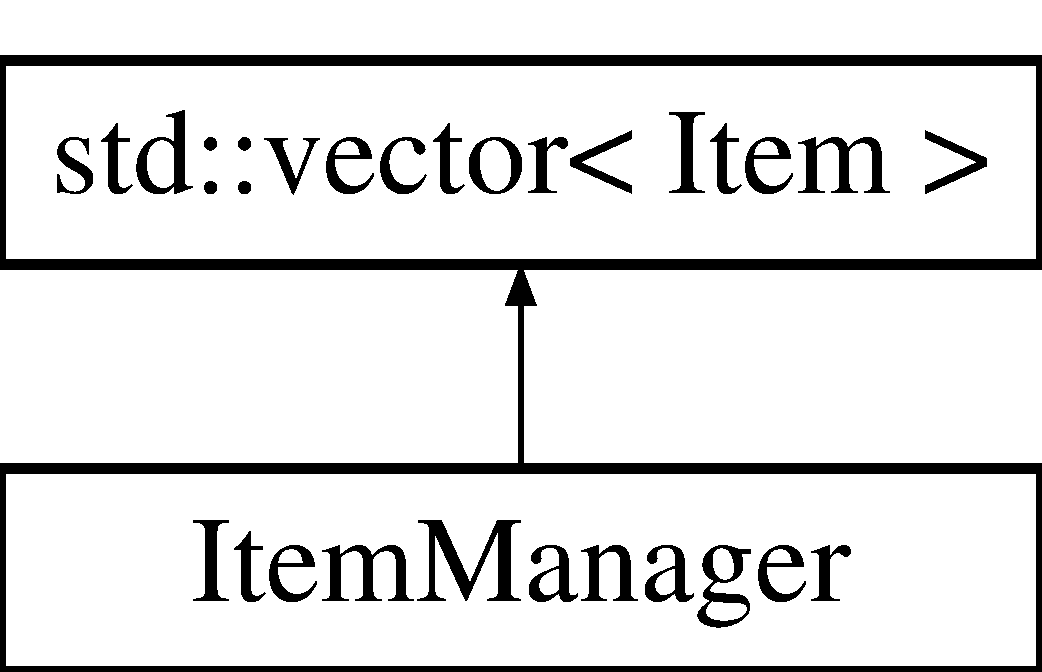
\includegraphics[height=2.000000cm]{classItemManager}
\end{center}
\end{figure}
\subsection*{Public Member Functions}
\begin{DoxyCompactItemize}
\item 
void \mbox{\hyperlink{classItemManager_ad3e190ba89c34cdaa4b11ecbdb6e8722}{display}} (std\+::ostream \&, bool=false) const
\end{DoxyCompactItemize}


\subsection{Detailed Description}
\mbox{\hyperlink{classItemManager}{Item\+Manager}} object that derives from a vector class of \mbox{\hyperlink{classItem}{Item}} type. 

\subsection{Member Function Documentation}
\mbox{\Hypertarget{classItemManager_ad3e190ba89c34cdaa4b11ecbdb6e8722}\label{classItemManager_ad3e190ba89c34cdaa4b11ecbdb6e8722}} 
\index{Item\+Manager@{Item\+Manager}!display@{display}}
\index{display@{display}!Item\+Manager@{Item\+Manager}}
\subsubsection{\texorpdfstring{display()}{display()}}
{\footnotesize\ttfamily void Item\+Manager\+::display (\begin{DoxyParamCaption}\item[{std\+::ostream \&}]{os,  }\item[{bool}]{full = {\ttfamily false} }\end{DoxyParamCaption}) const}

Member function that outputs item descriptions inside the base class. 

The documentation for this class was generated from the following files\+:\begin{DoxyCompactItemize}
\item 
Item\+Manager.\+h\item 
Item\+Manager.\+cpp\end{DoxyCompactItemize}

\hypertarget{classOrderManager}{}\section{Order\+Manager Class Reference}
\label{classOrderManager}\index{Order\+Manager@{Order\+Manager}}


{\ttfamily \#include $<$Order\+Manager.\+h$>$}

Inheritance diagram for Order\+Manager\+:\begin{figure}[H]
\begin{center}
\leavevmode
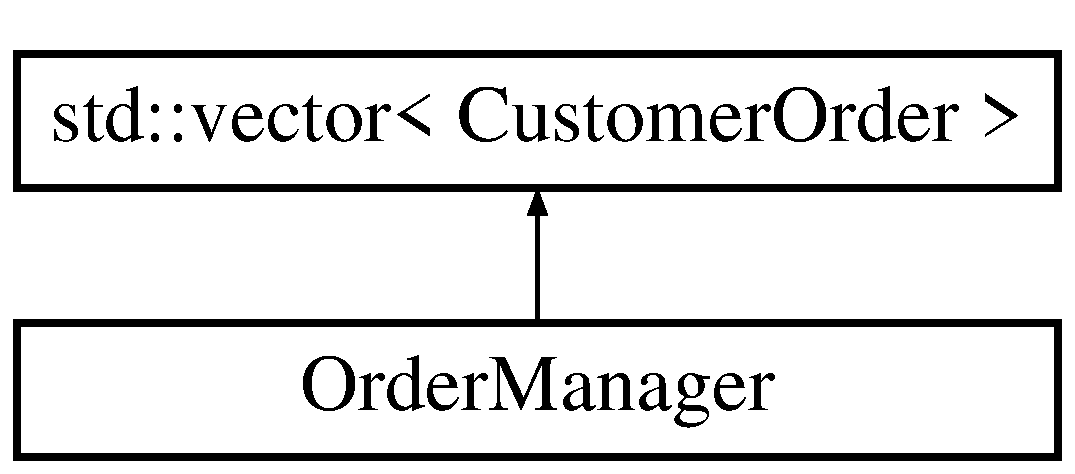
\includegraphics[height=2.000000cm]{classOrderManager}
\end{center}
\end{figure}
\subsection*{Public Member Functions}
\begin{DoxyCompactItemize}
\item 
\mbox{\hyperlink{classCustomerOrder}{Customer\+Order}} \&\& \mbox{\hyperlink{classOrderManager_a2111b67d23078421bb0c012c25ee87f1}{extract}} ()
\item 
void \mbox{\hyperlink{classOrderManager_a5469cae831246813134630f8bd85db79}{validate}} (const \mbox{\hyperlink{classItemManager}{Item\+Manager}} \&, std\+::ostream \&)
\item 
void \mbox{\hyperlink{classOrderManager_a01ff4be0afbb0535de41d5caedcf0016}{display}} (std\+::ostream \&) const
\end{DoxyCompactItemize}


\subsection{Detailed Description}
\mbox{\hyperlink{classOrderManager}{Order\+Manager}} object which derives from a vector class of datatype \mbox{\hyperlink{classCustomerOrder}{Customer\+Order}}. 

\subsection{Member Function Documentation}
\mbox{\Hypertarget{classOrderManager_a01ff4be0afbb0535de41d5caedcf0016}\label{classOrderManager_a01ff4be0afbb0535de41d5caedcf0016}} 
\index{Order\+Manager@{Order\+Manager}!display@{display}}
\index{display@{display}!Order\+Manager@{Order\+Manager}}
\subsubsection{\texorpdfstring{display()}{display()}}
{\footnotesize\ttfamily void Order\+Manager\+::display (\begin{DoxyParamCaption}\item[{std\+::ostream \&}]{os }\end{DoxyParamCaption}) const}

Member function that outputs the descriptions of each customer order inside the base class to the ostream object reference parametered. \mbox{\Hypertarget{classOrderManager_a2111b67d23078421bb0c012c25ee87f1}\label{classOrderManager_a2111b67d23078421bb0c012c25ee87f1}} 
\index{Order\+Manager@{Order\+Manager}!extract@{extract}}
\index{extract@{extract}!Order\+Manager@{Order\+Manager}}
\subsubsection{\texorpdfstring{extract()}{extract()}}
{\footnotesize\ttfamily \mbox{\hyperlink{classCustomerOrder}{Customer\+Order}} \&\& Order\+Manager\+::extract (\begin{DoxyParamCaption}{ }\end{DoxyParamCaption})}

Member function that moves a \mbox{\hyperlink{classCustomerOrder}{Customer\+Order}} from the back of the base class container and returns that object as an r valued object. \mbox{\Hypertarget{classOrderManager_a5469cae831246813134630f8bd85db79}\label{classOrderManager_a5469cae831246813134630f8bd85db79}} 
\index{Order\+Manager@{Order\+Manager}!validate@{validate}}
\index{validate@{validate}!Order\+Manager@{Order\+Manager}}
\subsubsection{\texorpdfstring{validate()}{validate()}}
{\footnotesize\ttfamily void Order\+Manager\+::validate (\begin{DoxyParamCaption}\item[{const \mbox{\hyperlink{classItemManager}{Item\+Manager}} \&}]{obj,  }\item[{std\+::ostream \&}]{os }\end{DoxyParamCaption})}

Member function that checks that the items requested are available. Appends a message if it is not available. 

The documentation for this class was generated from the following files\+:\begin{DoxyCompactItemize}
\item 
Order\+Manager.\+h\item 
Order\+Manager.\+cpp\end{DoxyCompactItemize}

\hypertarget{classTask}{}\section{Task Class Reference}
\label{classTask}\index{Task@{Task}}
\subsection*{Public Types}
\begin{DoxyCompactItemize}
\item 
\mbox{\Hypertarget{classTask_a6b8b1fc5858cbd77055e79d6381282fb}\label{classTask_a6b8b1fc5858cbd77055e79d6381282fb}} 
enum {\bfseries Quality} \{ {\bfseries passed}, 
{\bfseries redirect}
 \}
\end{DoxyCompactItemize}
\subsection*{Public Member Functions}
\begin{DoxyCompactItemize}
\item 
\mbox{\hyperlink{classTask_ace3ff25451f6d46f6cc0f2d7ed4b16ef}{Task}} (const std\+::string \&)
\item 
bool \mbox{\hyperlink{classTask_a974eb3143ac070fd67495f3c4a108a96}{validate}} (const \mbox{\hyperlink{classTask}{Task}} \&)
\item 
const std\+::string \& \mbox{\hyperlink{classTask_af12eb32f3bc744e6fa0480ca99c11f2c}{get\+Name}} () const
\item 
unsigned int \mbox{\hyperlink{classTask_a67589413dbb0d5ffa3b2f08c6fa461ea}{get\+Slots}} () const
\item 
const \mbox{\hyperlink{classTask}{Task}} $\ast$ \mbox{\hyperlink{classTask_acf6851078d506896872fa7cc6476e5bf}{get\+Next\+Task}} (Quality) const
\item 
void \mbox{\hyperlink{classTask_aff00aecd7c14bd02434b76ad10a656a2}{display}} (std\+::ostream \&) const
\end{DoxyCompactItemize}
\subsection*{Static Public Member Functions}
\begin{DoxyCompactItemize}
\item 
static size\+\_\+t \mbox{\hyperlink{classTask_a18f265f8b4a37e5ed047034c2558068b}{get\+Field\+Width}} ()
\end{DoxyCompactItemize}


\subsection{Constructor \& Destructor Documentation}
\mbox{\Hypertarget{classTask_ace3ff25451f6d46f6cc0f2d7ed4b16ef}\label{classTask_ace3ff25451f6d46f6cc0f2d7ed4b16ef}} 
\index{Task@{Task}!Task@{Task}}
\index{Task@{Task}!Task@{Task}}
\subsubsection{\texorpdfstring{Task()}{Task()}}
{\footnotesize\ttfamily Task\+::\+Task (\begin{DoxyParamCaption}\item[{const std\+::string \&}]{str }\end{DoxyParamCaption})}

Object constructor that uses a parametered constant reference to a string object to create a \mbox{\hyperlink{classTask}{Task}} object. 

\subsection{Member Function Documentation}
\mbox{\Hypertarget{classTask_aff00aecd7c14bd02434b76ad10a656a2}\label{classTask_aff00aecd7c14bd02434b76ad10a656a2}} 
\index{Task@{Task}!display@{display}}
\index{display@{display}!Task@{Task}}
\subsubsection{\texorpdfstring{display()}{display()}}
{\footnotesize\ttfamily void Task\+::display (\begin{DoxyParamCaption}\item[{std\+::ostream \&}]{os }\end{DoxyParamCaption}) const}

Member function that displays details of the current object. \mbox{\Hypertarget{classTask_a18f265f8b4a37e5ed047034c2558068b}\label{classTask_a18f265f8b4a37e5ed047034c2558068b}} 
\index{Task@{Task}!get\+Field\+Width@{get\+Field\+Width}}
\index{get\+Field\+Width@{get\+Field\+Width}!Task@{Task}}
\subsubsection{\texorpdfstring{get\+Field\+Width()}{getFieldWidth()}}
{\footnotesize\ttfamily static size\+\_\+t Task\+::get\+Field\+Width (\begin{DoxyParamCaption}{ }\end{DoxyParamCaption})\hspace{0.3cm}{\ttfamily [inline]}, {\ttfamily [static]}}

Member function that returns the field\+\_\+width of the current object. \mbox{\Hypertarget{classTask_af12eb32f3bc744e6fa0480ca99c11f2c}\label{classTask_af12eb32f3bc744e6fa0480ca99c11f2c}} 
\index{Task@{Task}!get\+Name@{get\+Name}}
\index{get\+Name@{get\+Name}!Task@{Task}}
\subsubsection{\texorpdfstring{get\+Name()}{getName()}}
{\footnotesize\ttfamily const std\+::string\& Task\+::get\+Name (\begin{DoxyParamCaption}{ }\end{DoxyParamCaption}) const\hspace{0.3cm}{\ttfamily [inline]}}

Member function that returns the name of the current \mbox{\hyperlink{classTask}{Task}}. \mbox{\Hypertarget{classTask_acf6851078d506896872fa7cc6476e5bf}\label{classTask_acf6851078d506896872fa7cc6476e5bf}} 
\index{Task@{Task}!get\+Next\+Task@{get\+Next\+Task}}
\index{get\+Next\+Task@{get\+Next\+Task}!Task@{Task}}
\subsubsection{\texorpdfstring{get\+Next\+Task()}{getNextTask()}}
{\footnotesize\ttfamily const \mbox{\hyperlink{classTask}{Task}} $\ast$ Task\+::get\+Next\+Task (\begin{DoxyParamCaption}\item[{Quality}]{quality }\end{DoxyParamCaption}) const}

Member function that returns a pointer to the next\+Task at the index of a parametered enum of this object. \mbox{\Hypertarget{classTask_a67589413dbb0d5ffa3b2f08c6fa461ea}\label{classTask_a67589413dbb0d5ffa3b2f08c6fa461ea}} 
\index{Task@{Task}!get\+Slots@{get\+Slots}}
\index{get\+Slots@{get\+Slots}!Task@{Task}}
\subsubsection{\texorpdfstring{get\+Slots()}{getSlots()}}
{\footnotesize\ttfamily unsigned int Task\+::get\+Slots (\begin{DoxyParamCaption}{ }\end{DoxyParamCaption}) const\hspace{0.3cm}{\ttfamily [inline]}}

Member function that returns the number of slots within the current \mbox{\hyperlink{classTask}{Task}} \mbox{\Hypertarget{classTask_a974eb3143ac070fd67495f3c4a108a96}\label{classTask_a974eb3143ac070fd67495f3c4a108a96}} 
\index{Task@{Task}!validate@{validate}}
\index{validate@{validate}!Task@{Task}}
\subsubsection{\texorpdfstring{validate()}{validate()}}
{\footnotesize\ttfamily bool Task\+::validate (\begin{DoxyParamCaption}\item[{const \mbox{\hyperlink{classTask}{Task}} \&}]{task }\end{DoxyParamCaption})}

Member function that recieves a constant reference to a \mbox{\hyperlink{classTask}{Task}} object and compares the parametered object to the current object\textquotesingle{}s next\+Task. 

The documentation for this class was generated from the following files\+:\begin{DoxyCompactItemize}
\item 
Task.\+h\item 
Task.\+cpp\end{DoxyCompactItemize}

\hypertarget{classTaskManager}{}\section{Task\+Manager Class Reference}
\label{classTaskManager}\index{Task\+Manager@{Task\+Manager}}


{\ttfamily \#include $<$Task\+Manager.\+h$>$}

Inheritance diagram for Task\+Manager\+:\begin{figure}[H]
\begin{center}
\leavevmode
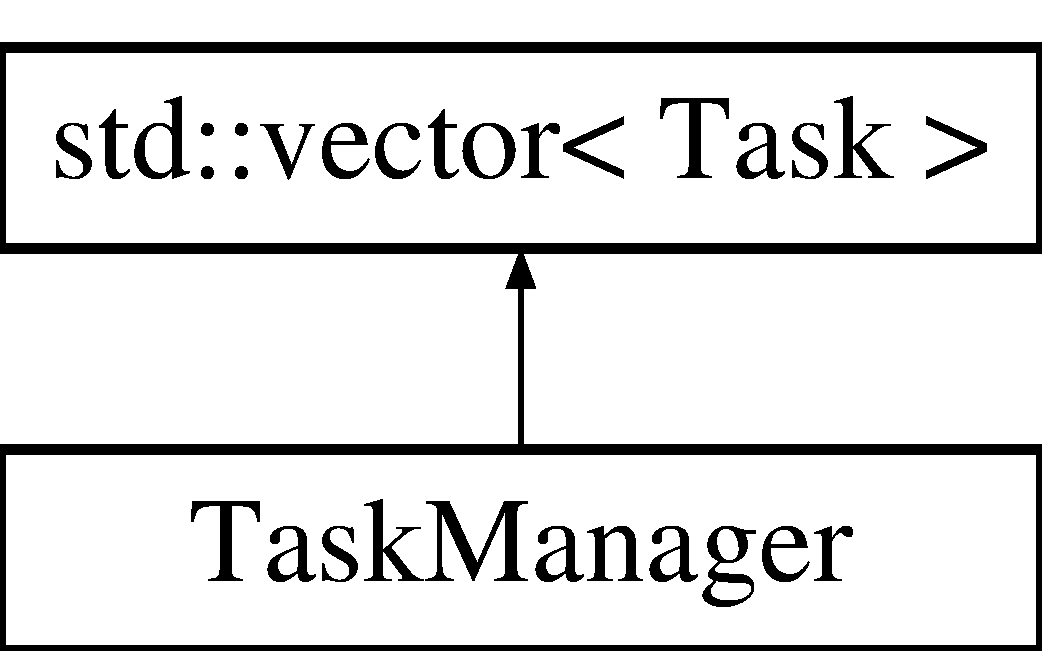
\includegraphics[height=2.000000cm]{classTaskManager}
\end{center}
\end{figure}
\subsection*{Public Member Functions}
\begin{DoxyCompactItemize}
\item 
void \mbox{\hyperlink{classTaskManager_a2ae3c30ca4e030440b64c383cbda8a73}{validate}} (std\+::ostream \&)
\item 
void \mbox{\hyperlink{classTaskManager_a59aea57b2ad273d6d95797f93d737fa0}{validate}} (const \mbox{\hyperlink{classItemManager}{Item\+Manager}} \&, std\+::ostream \&)
\item 
void \mbox{\hyperlink{classTaskManager_a3564901af8fa7498b0fcca85fcaa5e64}{display}} (std\+::ostream \&) const
\end{DoxyCompactItemize}


\subsection{Detailed Description}
\mbox{\hyperlink{classTaskManager}{Task\+Manager}} object that manages it\textquotesingle{}s vector object base class populated with \mbox{\hyperlink{classTask}{Task}} objects. 

\subsection{Member Function Documentation}
\mbox{\Hypertarget{classTaskManager_a3564901af8fa7498b0fcca85fcaa5e64}\label{classTaskManager_a3564901af8fa7498b0fcca85fcaa5e64}} 
\index{Task\+Manager@{Task\+Manager}!display@{display}}
\index{display@{display}!Task\+Manager@{Task\+Manager}}
\subsubsection{\texorpdfstring{display()}{display()}}
{\footnotesize\ttfamily void Task\+Manager\+::display (\begin{DoxyParamCaption}\item[{std\+::ostream \&}]{os }\end{DoxyParamCaption}) const}

Member function that outputs descriptions of the tasks stored in the base class. \mbox{\Hypertarget{classTaskManager_a2ae3c30ca4e030440b64c383cbda8a73}\label{classTaskManager_a2ae3c30ca4e030440b64c383cbda8a73}} 
\index{Task\+Manager@{Task\+Manager}!validate@{validate}}
\index{validate@{validate}!Task\+Manager@{Task\+Manager}}
\subsubsection{\texorpdfstring{validate()}{validate()}\hspace{0.1cm}{\footnotesize\ttfamily [1/2]}}
{\footnotesize\ttfamily void Task\+Manager\+::validate (\begin{DoxyParamCaption}\item[{std\+::ostream \&}]{os }\end{DoxyParamCaption})}

Member function that validates a task against all tasks inside the base class and appends a message if it is not validated. \mbox{\Hypertarget{classTaskManager_a59aea57b2ad273d6d95797f93d737fa0}\label{classTaskManager_a59aea57b2ad273d6d95797f93d737fa0}} 
\index{Task\+Manager@{Task\+Manager}!validate@{validate}}
\index{validate@{validate}!Task\+Manager@{Task\+Manager}}
\subsubsection{\texorpdfstring{validate()}{validate()}\hspace{0.1cm}{\footnotesize\ttfamily [2/2]}}
{\footnotesize\ttfamily void Task\+Manager\+::validate (\begin{DoxyParamCaption}\item[{const \mbox{\hyperlink{classItemManager}{Item\+Manager}} \&}]{obj,  }\item[{std\+::ostream \&}]{os }\end{DoxyParamCaption})}

Member function that tasks to handle the \mbox{\hyperlink{classItemManager}{Item\+Manager}} object reference exist within the base class. Appends a message if the task does not exist. 

The documentation for this class was generated from the following files\+:\begin{DoxyCompactItemize}
\item 
Task\+Manager.\+h\item 
Task\+Manager.\+cpp\end{DoxyCompactItemize}

\hypertarget{classUtilities}{}\section{Utilities Class Reference}
\label{classUtilities}\index{Utilities@{Utilities}}
\subsection*{Public Member Functions}
\begin{DoxyCompactItemize}
\item 
\mbox{\hyperlink{classUtilities_ab1676c9ce35cf347a73d16f1094e1271}{Utilities}} ()
\item 
size\+\_\+t \mbox{\hyperlink{classUtilities_a94abc3ceade71097979e76e15008efba}{get\+Field\+Width}} () const
\item 
const std\+::string \mbox{\hyperlink{classUtilities_a59c27deae1e3810d8591b35ed90b7f33}{next\+Token}} (const std\+::string \&, size\+\_\+t \&, bool \&)
\end{DoxyCompactItemize}
\subsection*{Static Public Member Functions}
\begin{DoxyCompactItemize}
\item 
static void \mbox{\hyperlink{classUtilities_a833c24f770f9bd4c128cfc9dabb60a29}{set\+Delimiter}} (const char c)
\item 
static void \mbox{\hyperlink{classUtilities_a63a49d3b5ff70602f519d045234e7992}{set\+Log\+File}} (const char $\ast$name)
\item 
static std\+::ofstream \& \mbox{\hyperlink{classUtilities_aecd7de50b27a709a9810b17940074cad}{get\+Log\+File}} ()
\end{DoxyCompactItemize}


\subsection{Constructor \& Destructor Documentation}
\mbox{\Hypertarget{classUtilities_ab1676c9ce35cf347a73d16f1094e1271}\label{classUtilities_ab1676c9ce35cf347a73d16f1094e1271}} 
\index{Utilities@{Utilities}!Utilities@{Utilities}}
\index{Utilities@{Utilities}!Utilities@{Utilities}}
\subsubsection{\texorpdfstring{Utilities()}{Utilities()}}
{\footnotesize\ttfamily Utilities\+::\+Utilities (\begin{DoxyParamCaption}{ }\end{DoxyParamCaption})}

Default constructor sets object to empty state with field width of 1. 

\subsection{Member Function Documentation}
\mbox{\Hypertarget{classUtilities_a94abc3ceade71097979e76e15008efba}\label{classUtilities_a94abc3ceade71097979e76e15008efba}} 
\index{Utilities@{Utilities}!get\+Field\+Width@{get\+Field\+Width}}
\index{get\+Field\+Width@{get\+Field\+Width}!Utilities@{Utilities}}
\subsubsection{\texorpdfstring{get\+Field\+Width()}{getFieldWidth()}}
{\footnotesize\ttfamily size\+\_\+t Utilities\+::get\+Field\+Width (\begin{DoxyParamCaption}{ }\end{DoxyParamCaption}) const\hspace{0.3cm}{\ttfamily [inline]}}

Member function that returns the field\+\_\+width of this object. \mbox{\Hypertarget{classUtilities_aecd7de50b27a709a9810b17940074cad}\label{classUtilities_aecd7de50b27a709a9810b17940074cad}} 
\index{Utilities@{Utilities}!get\+Log\+File@{get\+Log\+File}}
\index{get\+Log\+File@{get\+Log\+File}!Utilities@{Utilities}}
\subsubsection{\texorpdfstring{get\+Log\+File()}{getLogFile()}}
{\footnotesize\ttfamily static std\+::ofstream\& Utilities\+::get\+Log\+File (\begin{DoxyParamCaption}{ }\end{DoxyParamCaption})\hspace{0.3cm}{\ttfamily [inline]}, {\ttfamily [static]}}

Static member function that retrieves a reference to a std\+::ofstream object. \mbox{\Hypertarget{classUtilities_a59c27deae1e3810d8591b35ed90b7f33}\label{classUtilities_a59c27deae1e3810d8591b35ed90b7f33}} 
\index{Utilities@{Utilities}!next\+Token@{next\+Token}}
\index{next\+Token@{next\+Token}!Utilities@{Utilities}}
\subsubsection{\texorpdfstring{next\+Token()}{nextToken()}}
{\footnotesize\ttfamily const std\+::string Utilities\+::next\+Token (\begin{DoxyParamCaption}\item[{const std\+::string \&}]{str,  }\item[{size\+\_\+t \&}]{next\+\_\+pos,  }\item[{bool \&}]{more }\end{DoxyParamCaption})}

Member function that retrives a reference to a string to parse, a reference to a size\+\_\+t datatype to reference a position of where in the string to begin parsing, a reference to a bool datatype to flag whether or not parsing can be continued. This member function returns the parsed token referenced by a parametered string reference. \mbox{\Hypertarget{classUtilities_a833c24f770f9bd4c128cfc9dabb60a29}\label{classUtilities_a833c24f770f9bd4c128cfc9dabb60a29}} 
\index{Utilities@{Utilities}!set\+Delimiter@{set\+Delimiter}}
\index{set\+Delimiter@{set\+Delimiter}!Utilities@{Utilities}}
\subsubsection{\texorpdfstring{set\+Delimiter()}{setDelimiter()}}
{\footnotesize\ttfamily static void Utilities\+::set\+Delimiter (\begin{DoxyParamCaption}\item[{const char}]{c }\end{DoxyParamCaption})\hspace{0.3cm}{\ttfamily [inline]}, {\ttfamily [static]}}

Static member function that sets the delimiter when string parsing. \mbox{\Hypertarget{classUtilities_a63a49d3b5ff70602f519d045234e7992}\label{classUtilities_a63a49d3b5ff70602f519d045234e7992}} 
\index{Utilities@{Utilities}!set\+Log\+File@{set\+Log\+File}}
\index{set\+Log\+File@{set\+Log\+File}!Utilities@{Utilities}}
\subsubsection{\texorpdfstring{set\+Log\+File()}{setLogFile()}}
{\footnotesize\ttfamily static void Utilities\+::set\+Log\+File (\begin{DoxyParamCaption}\item[{const char $\ast$}]{name }\end{DoxyParamCaption})\hspace{0.3cm}{\ttfamily [inline]}, {\ttfamily [static]}}

Static member function that closes an open std\+::ofstream object and creates a new std\+::ofstream object from the character array paramatered to this function. 

The documentation for this class was generated from the following files\+:\begin{DoxyCompactItemize}
\item 
Utilities.\+h\item 
Utilities.\+cpp\end{DoxyCompactItemize}

%--- End generated contents ---

% Index
\backmatter
\newpage
\phantomsection
\clearemptydoublepage
\addcontentsline{toc}{chapter}{Index}
\printindex

\end{document}
